\chapter{Fusing Acoustic and Linguistic Information at Feature Level}
\chaptermark{Feature-level Fusion}
This chapter evaluates the fusion of acoustic and linguistic information at the
feature level. Two approaches were evaluated, network concatenation and feature
concatenation. A comparison of manual and automatic transcriptions from the
IEMOCAP dataset provides insight into the current automatic speech recognition
system's contribution to speech emotion recognition (SER).

% \section{Introduction}
\section{Extracting linguistic information}

\subsection{Word embeddings}
A classifier needs a set of input features to model input-output relation. One
of the common features used in text processing is word embeddings or word
vectors. A word embedding is a vector representation of a word. A numerical
value in the form of a vector is used to make the computer to be able to
process text data as it only processes numerical values. This value is the
points (numeric data) in the space of a dimension, in which the size of the
dimension is equal to the vocabulary size.  The word representations embed
these points in a feature space of lower dimension
\cite{IanGoodfellowYoshuaBengio2015}. A one-hot vector represents every word; a
value of 1 corresponds to this word and 0 for others.  This element with a
value of 1 will be converted into a point in the range of vocabulary size.

To obtain a vector of each word in an utterance, first, this utterance in the
dataset must be tokenized. Tokenization is a process to divide an utterance by
the number of constituent words. For example, the text "That's out of control."
from IEMOCAP dataset will be tokenized as [``That's," ``out," ``of,"
``control"].  Suppose the number of vocabulary is 2182 (number of words in
IEMOCAP dataset with six emotion categories), then the obtained word vector is
something similar to

\begin{verbatim}
 text_vector = [42, 44, 11, 471].
\end{verbatim}

% \begin{verbatim} vocab_size = 50 text = ["That's out of control"] text -->
% vector output vector = [43, 41, 4, 5] \end{verbatim}
An embedding layer will convert those positive fixed integers into dense
vectors of fixed size. For instance, 1-dimensional word vector in the utterance
will be converted into 2-dimensional dense vector,
\begin{equation*}
    [42, 44, 11, 471] \rightarrow  [[0.12, 0.3], [0.12, 0.29], [-0.54, 0.2], [0.71, 0.23]].
\end{equation*}

The higher dimensions are commonly used to obtain a better representation of a
word vector. A number of 50-, 100-, and 300-dimensional vectors are commonly
employed to build pre-trained word vectors from a large corpus.

% The vector obtained above might be different in each computation process. 
A set of zeros can be padded in front of or behind the obtained vector to
obtain the fixed-length vector for all utterances. The size of this zeros
sequence can be obtained from the longest sequence, i.e., an utterance within
the dataset which has the longest words, subtracted by the length of a vector
in the current utterance.


\subsection{Pre-trained word embeddings}

A study to vectorize certain words has been performed by several researchers
\cite{Mikolov, Pennington2014, Mikolov2019}. The vector of those words can be
used to weight the word vector obtained previously. The following pre-trained
word embedding models were used in this research. \\

\noindent \textbf{word2vec} \\
Classical word embedding paradigm used unsupervised (hand-crafted) learning
algorithms, such as LSA, n-gram, and TF-IDF. Due to advancements in neural
network theory supported by computer hardware's speedup, word vector search
shifted to deep learning-based algorithms. Mikolov et al. \cite{Mikolov}
developed word representation using the so-called word2vec (word to vector)
using a neural network language model trained in two steps. First, continuous
word vectors are learned by using a simple model, and then the n-gram neural
net language model (NNLM) is trained on top of these distributed
representations of words \cite{Mikolov}. Two new model architectures are
proposed to obtain word vector: the Continuous-Bag-of-Word (CBOW) architecture
to predict the current word based on the context. The skip-gram predicts
surrounding words given the current word. Figure \ref{fig:word2vec} shows those
two different architectures and how they process the input to the output.

\begin{figure}
\centering
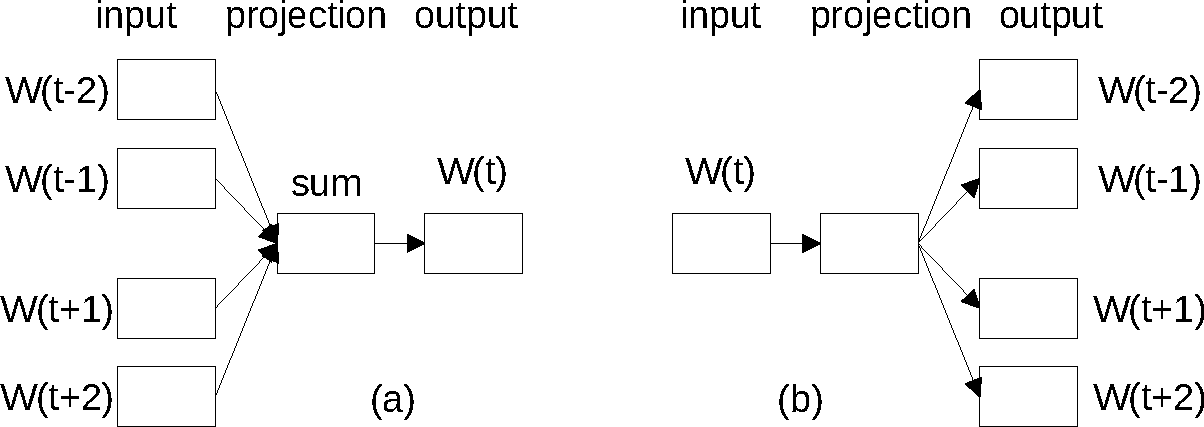
\includegraphics[width=4in]{../fig/word2vec-crop.pdf}
\caption{Two architectures of word2vec: (a) CBOW and (b) skip-gram \cite{Mikolov}}
\label{fig:word2vec}
\end{figure}

From those two approaches, skip-gram was founded as an efficient method for
learning high-quality distributed vector representations that capture precise
syntactic and semantic word relationships \cite{Mikolov}. The objective of the
skip-gram model is to maximize the average log probability,

\begin{equation}
\dfrac{1}{T}\sum_{t=1}^{T}\sum_{-c<j<c, c\neq0}\log p(w_{t+j}|w_t),
\label{eq:skipgram}
\end{equation}

\noindent where $c$ is the size of the training context (which can be a
function of the center word $w_t$). Larger $c$ results in more training
examples and can lead to higher accuracy, at the expense of the training time.
The basic skip-gram formulation of $p(w_{t+j} |w_t)$ can be defined using the
softmax function, and computational efficiency can be approached by a
hierarchical softmax \cite{Mikolov}. \\

\noindent \textbf{GloVe} \\
Pennington et al. \cite{Pennington2014} combined global matrix factorization
and local context window methods for learning the space representation of a
word.  In GloVe (Global Vectors) model, the statistics of word occurrences in a
corpus are the primary source of information available to all unsupervised
methods for learning the word representations. Although man methods now exist,
the question remains as to how meaning is generated from these statistics and
how the resulting word vectors might represent that meaning. Glove captured the
global statistics from the corpus, for example, a Wikipedia document or a
common crawl document. 

In GloVe model, the cost function is given by
\begin{equation}
\sum_{i,j=1}^{V}f(X_{i,j})(u_{i,j}^Tv_j+b_i+c_j-\log X_{i,j})^2,
\label{eq:glove}
\end{equation}

\noindent where
\begin{itemize}
\item $V$ is the size of the vocabulary;
\item $X$ denotes the word co-occurrence matrix (so $X_{i,j}$ is the number of
times that word j occurs in the context of word i);
\item the weighting $f$ is given by $f(x) = (x / x_{\text{max}})^\alpha$ if $x
< x_{\text{max}}$ and 1 otherwise;
\item $x_{\text{max}} = 100$ and $\alpha = 0.75$ (determined empirically);
\item $u_i$, $v_j$ are the two layers of word vectors;
\item $b_i$, $c_j$ are bias terms.
\end{itemize}

\noindent In a simple way, GloVe is a weighted matrix factorization with the
bias terms, as shown in Figure \ref{fig:glove}. \\

\begin{figure}
\centering
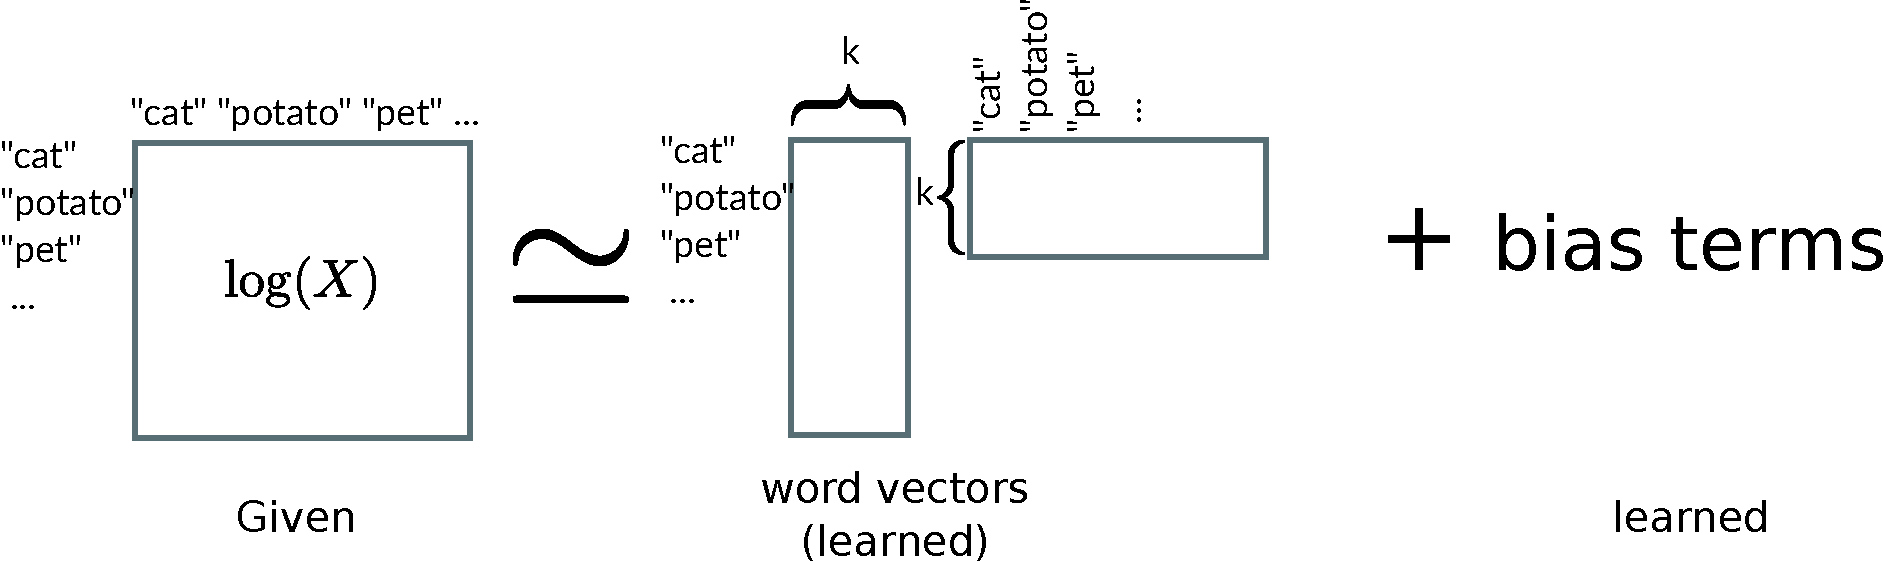
\includegraphics[width=5in]{../fig/glove.pdf}
\caption{Illustration of GloVe representation}
\label{fig:glove}
\end{figure}

\noindent \textbf{FastText} \\
Mikolov et al. \cite{Mikolov2019} improved word2vec CBOW model by using some
strategies including subsample frequent words technique. This modification of
word2vec is trained on large text corpus, such as news collection, Wikipedia,
and web crawl. They named the pre-trained model with that modification as
FastText.  The following probability $p_{disc}$ of discarding a word is used by
FastText to subsample the frequent words:

\begin{equation}
P_{disc} (w) = 1 - \sqrt{t/f_w},
\label{eq:fastext}
\end{equation}

\noindent where $f_w$ is the frequency of the word $w$, and t is a parameter
$>$ 0.

FastText also counts the classical n-gram word representation by enriching word
vector with a bag of character n-gram vectors learned from a large corpus. In
this computation, each word is decomposed into its character n-grams $N$, and
each n-gram $n$ is represented by a vector $x_n$. The new word vector is then
simply the sum of both representations,

\begin{equation}
v_w + \dfrac{1}{|N|} \sum_{n\in N}x_n,
\label{eq:subword}
\end{equation}

\noindent where $v_w$ is the old word vector. The set of n-grams $N$ is limited
to 3 to 6 characters in practical implementation. \\


\noindent \textbf{BERT} \\
The previous aforementioned word embeddings --- word2vec, GloVe, FastText ---
are generated word representation in a context-free model. It means, the same
word appears in a different phrase has the same word representation, e.g., word
``book'' in ``mathematics book" and ``book a hotel." Instead of using a
context-free model, BERT (bidirectional transformers language understanding)
was built upon pre-training contextual representation \cite{Devlin2018}.

BERT is different in many ways from its predecessors. Apart from contextual
representation, the main contribution of BERT is to employ bidirectional
pre-training for language representation. Unlike its predecessors, which model
languages in a unidirectional way, i.e., from left to right as a
writing/reading system, BERT used two unsupervised tasks for pre-training
models. The first task is the masked language model; the second task is the
next sentence prediction (NSP). The BERT model's dimension for each word
depends on the number of hidden layers used in the architecture. This number is
either 768-dimensions for the base model, or 1024-dimension for the large
model.

Apart from the pre-trained model, BERT provides a fine-tuning model.
Fine-tuning allows BERT to model several tasks, single or text pairs, by
swapping out the corresponding inputs and outputs. Fine-tuning can be seen as
adjusting the pre-trained model according to the context, i.e., the dataset.
Hence, fine-tuning can only be done after obtaining the pre-trained model and
is relatively expensive. Fine-tuning is suitable for a specific task rather
than general linguistic tasks.

\subsection{CCC loss function}

In the Chapter 3, a metric to measure the performance of dimensional emotion
recognition was introduced, namely concordance correlation coefficient. Since,
the goal is CCC, using CCC loss instead of conventional regression loss
function such as mean square error (MSE) and mean absolute error (MAE) is more
beneficial than both error-based loss functions.  The CCC loss function (CCCL)
to maximize the agreement between the true value and the predicted emotion can
be defined as 
\begin{equation}
 CCCL = 1 - CCC.
\end{equation}
In single-task learning, the loss function would be one for either valence
($CCCL_{V}$), arousal ($CCCL_{A}$), or dominance ($CCCL_{D}$). In multitask
learning (MTL), when the total CCC loss is used as a single metric for
predicting valence, arousal, and dominance simultaneously, $CCCL_{tot}$ is the
following combination of those three CCC loss functions:
\begin{equation}
 CCCL_{tot} = CCCL_{V} + CCCL_{A} + CCCL_{D}.
\label{eq:mtl}
\end{equation}

\noindent This MTL equation is referred as ``MTL without parameters,'' because
there is no weighting among valence, arousal, and dominance. In this case, the
relation among the three emotional dimensions is determined by joint learning
in the training process. As it has been stated that these three emotional
dimensions are related in a systemic manner \cite{Gunes2010}, two parameters
are introduced to weight the valence and arousal, with the weight for dominance
determined by subtracting those two parameters from 1. This MTL with two
parameters is defined as
\begin{align}
\begin{split}
 CCCL_{tot} =& ~ \alpha ~ CCCL_{V} + \beta ~ CCCL_{A} \\
 &+ (1-\alpha-\beta) ~ CCCL_{D},
\label{eq:mtl-2}
\end{split}
\end{align}
where $\alpha$ and $\beta$ are the weighting factors for the valence and
arousal loss functions, respectively. This proposed MTL is similar to that
defined in \cite{parthasarathy2017jointly}. While those authors used the mean
squared error (MSE) as the loss function, this study have proposed using this
CCC-based loss function. In addition, a parameter $\gamma$ is added for
dominance to obtain independent scales among valence, arousal, and dominance.
The resulting MTL with three parameters is defined as 
\begin{equation}
 CCCL_{tot} = \alpha ~ CCCL_{V} + \beta ~ CCCL_{A} + \gamma ~ CCCL_{D}.
\label{eq:mtl-3}
\end{equation}
For comparison with the previous MTL without parameters; $\alpha$, $\beta$, and
$\gamma$ were set to 1 in that equation \ref{eq:mtl}, which can be seen as a
special case in this MTL with three parameters.

These MTL approaches compare the predicted output from the three one-unit dense
layers with the ground truth labels. The training process mechanism relies on
the above loss function. Hence, the performance of the produced model is based
on this mechanism, too. The loss function's choice is a critical aspect of
machine learning, and this study thus proposed this MTL based on the CCC loss
to learn valence, arousal, and dominance concurrently.

\section{Early fusion by networks concatenation}
A simple way to fuse two different information is by concatenating two DNNs of
different network modalities. Different shape of features is not a problem in
this fusion; the concatenation branch only requires the same dimension of DNN
outputs from each network. For instance, a 3D vector can solely be concatenated
with another 3D vector.

A unimodal feature is a feature set from either acoustic or linguistic (e.g.,
pAA LLD). At first, the system trained each feature set on both LSTM and CNN
classifiers independently. Tables \ref{tab:acoustic-result} and
\ref{tab:text-result} summarize the unimodal dimensional emotion results from
those acoustic and linguistic networks, respectively. Each table lists the
scores for valence, arousal, and dominance in terms of the CCC, along with
averaged CCC scores to determine which method performed better. The results
were grouped by modality and architecture. They all used the same metric scale
and were obtained under the same conditions. Hence, these results can be
compared directly with each other.

In the acoustic-based modality, the obtained results are consistent among the
feature sets on both architectures. From bottom to top, the performance order
was pAA LLD, GeMAPS LLD, GeMAPS HSF, and pAA HSF. Thus, although GeMAPS
performed better for LLDs, the HSF for pAA performed best on both the LSTM and
CNN architectures.  This result supports the previous finding that the mean and
standard deviation outperform the low-level descriptors (LLDs) defined in
GeMAPS. Furthermore, this finding can be generalized to the means and standard
deviations from the other feature sets. In this case, the HSF for pAA performed
better than the HSF for the affective-designed GeMAPS. 

Comparing the LSTM and CNN architectures, it is found that the LSTM performed
better than CNN did. In terms of three emotional dimensions and an average of
three, the score obtained by the highest-performing LSTM was higher than that
obtained by the highest-performing CNN. The best architecture in the acoustic
networks was chosen to combine with the linguistic networks' best
architectures.

As for the linguistic networks, word embeddings with the pre-trained GloVe
embeddings performed better than either word embeddings without weighting or
word embeddings weighted by the FastText model did. The linguistic networks
also showed that the LSTM with GloVe embedding is better than the CNN with the
same input feature. However, in this dimensional emotion recognition, the
linguistic network's highest performance was lower than an acoustic network's
highest performance. As with the acoustic networks, two networks were chosen,
GloVe with LSTM and GloVe with CNN, to combine in the bimodal network fusion. 

\begin{table}[htpb]
  \caption{CCC score results on the acoustic networks}
  \begin{center}
 \label{tab:acoustic-result}
 \begin{tabular}{l c c c c}
 \hline 
Feature set & V & A & D & Mean \\
\hline \hline
\multicolumn{5}{c}{LSTM} \\
pAA LLD & 0.0987 & 0.5175 & 0.3536 & 0.3233 \\
pAA HSF & 0.1729 & \textbf{0.5804} & \textbf{0.4476} & \textbf{0.4003} \\
GeMAPS LLD & 0.1629 & 0.5070 & 0.4433 & 0.3711 \\
GeMAPS HSF & \textbf{0.1818} & 0.5306 & 0.4332 & 0.3819 \\
 \hline
\multicolumn{5}{c}{CNN} \\ 
pAA LLD & 0.0687 & 0.3665 & 0.3382 & 0.2578 \\
pAA HSF & \textbf{0.1310} & \textbf{0.5553} & \textbf{0.4431} & \textbf{0.3764}
\\
GeMAPS LLD & 0.0581 & 0.4751 & 0.4203 & 0.3178 \\
GeMAPS HSF & 0.0975 & 0.4658 & 0.4170 & 0.3268 \\
 \hline
 \end{tabular}
\end{center}
\end{table} 

\begin{table}[htpb]
  \caption{CCC score results on the linguistic networks}
  \begin{center}
 \label{tab:text-result}
 \begin{tabular}{l c c c c}
 \hline
Feature set & V & A & D & Mean \\
\hline \hline
\multicolumn{5}{c}{LSTM} \\ 
WE       & 0.3784  & 0.3412 & 0.3638 & 0.3611 \\
word2vec & 0.3937  & 0.3811  & 0.3824  & 0.3857 \\
GloVe    & \textbf{0.4096} & \textbf{0.3886} & \textbf{0.3790} &
\textbf{0.3924} \\
FastText & 0.4017 & 0.3718 & 0.3771 & 0.3835 \\
BERT     & 0.3858  & 0.3675  & 0.3722  & 0.3752 \\
 \hline
\multicolumn{5}{c}{CNN} \\
WE       & 0.3740 & 0.3285 & 0.3144 & 0.3390 \\
word2vec & 0.3692  & 0.3589  & 0.3613  & 0.3631 \\
GloVe    & \textbf{0.3843} & 0.3646 & \textbf{0.3911} & \textbf{0.3800} \\
FastText & 0.3786 & \textbf{0.3648} & 0.3147 & 0.3527 \\
BERT     & 0.3598  & 0.3479  & 0.3530  & 0.3535 \\
 \hline
 \end{tabular}
\end{center}
\end{table} 

\subsection{Results on bimodal feature fusion}
\subsubsection{Performance of bimodal networks}
According to their unimodal network performance, eight pairs of bimodal
acoustic-linguistic networks were evaluated. Table \ref{tab:bimodal-result}
summarizes their performance results in the same way as the unimodal
results.  Among the eight pairs, the LSTM acoustic networks and the LSTM
linguistic networks achieved the best performance. This result in bimodal
feature fusion is linear with respect to the obtained results for the unimodal
networks, in which the LSTM performed best on both the acoustic and linguistic
networks. 

In terms of both emotional dimensions and average CCC scores, the LSTM+LSTM
pair outperformed the other bimodal pairs. Moreover, the deviation of the
LSTM+LSTM pair was also the lowest. It can be stated that, apart from attaining
the highest performance, the LSTM+LSTM pair also gave the most stable results.
This result suggests that the LSTM not only attained comparable results to the
CNN with a similar number of trainable parameters but also attained better
performances, which differs from what was reported in \cite{Schmitt2019}.

One reasonable explanation for why the LSTM performs better is the use of the
full sequence instead of the final sequence in the last LSTM layer. In most
applications, the last layer in an LSTM stack only returns the final sequence
to be combined with the outputs of other layers (e.g., a dense layer). In this
implementation, however, all sequences outputs were returned from the last LSTM
layer and flattened before combining them with another dense layer's output
(from the linguistic network). This strategy may keep more relevant information
than what is returned by the final sequence of the last LSTM layer. On the
other hand, this phenomenon is only observed on the acoustic network. In the
linguistic network case, the last LSTM layer that returns the final sequence
performed better than the LSTM that returns all sequences. In that latter case,
the last LSTM layer was directly coupled with that of a dense layer.

If the highest unimodal score is chosen as a baseline, i.e., the HSF of pAA,
then the highest bimodal score's relative improvement was 23.97\%. A
significance test among the bimodal pair results was performed. A significant
difference was observed between an LSTM+LSTM pair and other pairs, such as a
CNN+LSTM pair, on a two-tail paired test. The small $p$-value ($\simeq
10^{-5}$) indicated the strong difference obtained by the LSTM+LSTM and
CNN+LSTM pairs.  While the CNN+LSTM pair obtained the third-highest score, the
second-best performance was by a Dense+CNN pair with CCC = 0.485. The
significance test result between the LSTM+LSTM pair and this pair was $p$ =
0.0006. The more similar the performance of two acoustic-linguistic networks
pairs was, the higher the $p$-value between them was. The assertion that the
LSTM+LSTM pair had a big difference from the other pairs was set with $p <
0.05$.

\begin{table*}[htpb]
 \begin{center}
\caption{Results of bimodal feature fusion (without parameters) by
concatenating the acoustic and linguistic networks; each modality used either an
LSTM, CNN, or dense network; batch size = 8}
 \label{tab:bimodal-result}
 \begin{tabular}{l c c c c} 
 \hline
Acoustic+Linguistic & V & A & D & Mean\\
\hline \hline
LSTM + LSTM & \textbf{0.418 $\pm$ 0.01} & \textbf{0.571 $\pm$ 0.017} &
\textbf{0.5 $ \pm$ 0.017} & \textbf{0.496 $\pm$ 0.01} \\
LSTM + CNN & 0.256 $\pm$ 0.052 & 0.531 $\pm$ 0.031 & 0.450 $ \pm$ 0.036 & 0.412
$\pm$ 0.030 \\
CNN + LSTM & 0.401 $\pm$ 0.020 & 0.545 $\pm$ 0.016 & 0.478 $ \pm$ 0.015 & 0.476
$\pm$ 0.012 \\
CNN + CNN & 0.399 $\pm$ 0.015 & 0.541 $\pm$ 0.020 & 0.475 $ \pm$ 0.014 & 0.472
$\pm$ 0.012 \\
LSTM + Dense & 0.274 $\pm$ 0.050 & 0.553 $\pm$ 0.019 & 0.484 $ \pm$ 0.015 &
0.437 $\pm$ 0.018 \\
CNN + Dense & 0.266 $\pm$ 0.038 & 0.497 $\pm$ 0.059 & 0.457 $ \pm$ 0.047 &
0.407 $\pm$ 0.040 \\
Dense + LSTM & 0.368 $\pm$ 0.105 & 0.564 $\pm$ 0.015 & 0.478 $ \pm$ 0.025 &
0.470 $\pm$ 0.043 \\
Dense + CNN & 0.398 $\pm$ 0.015 & 0.570 $\pm$ 0.013 & 0.487 $ \pm$ 0.015 &
0.485 $\pm$ 0.013 \\
 \hline
 \end{tabular}
 \end{center}
\end{table*}

\subsubsection{Evaluation of MTL with weighting factors}
As an extension of the main proposal to jointly learn the valence, arousal, and
dominance from acoustic features and word embeddings by using MTL, this study
also evaluated some weighting factors for the MTL formulation (equations 4, 5,
and 6). In contrast, the above results were obtained using MTL with no
parameters (equation \ref{eq:mtl}). Thus, the following results show the effect
of the weighting parameters on the MTL method.

MTL with two parameters is an approach to capture the interrelation among
valence, arousal, and dominance. In equation \ref{eq:mtl-2}, the gains of
valence and arousal are provided independently, while the gain of dominance
depends on the other gains. This simple weighting strategy may represent the
relation among the emotional dimensions if the obtained results are better than
the results without this weighting strategy.

Figure \ref{fig:ccc_2-params} shows a surface plot of the impact of varying
$\alpha$ and $\beta$ from 0.0 to 1.0 with the corresponding average CCC score.
Performance improvement could be obtained by using proper weighting factors in
two-parameter MTL. It is found that $\alpha=0.7$ and $\beta=0.2$ were the best
weighting factors, and the linguistic network also used them.  In the unimodal
network, the best factors for MTL with two parameters were $\alpha=0.7$ and
$\beta=0.2$ for the linguistic networks, and $\alpha=0.1$ and $\beta=0.5$ for
the acoustic network. These factors were used to obtain the above unimodal results. In this case, it is difficult to judge whether these same obtained
factors for the bimodal network were contributed by the unimodal network or
caused by other factors.  Investigation on the cause of this finding is a
challenging issue for both theoretical and empirical studies.

Next, MTL with three parameters provided all factors for the three-dimensional
emotions, with every emotional dimension's factor is independent of each
other.  MTL with no parameters is also a subset of MTL with three parameters,
with $\alpha=1.0$, $\beta=1.0$, and $\gamma=1.0$. The experiments optimized the
weighting factors with three parameters by using linear search independently on
each emotion dimension. Figure \ref{fig:ccc_3-params} shows the impact of the
weighting factors on MTL with three parameters. In this scaling strategy, the
best weighting factors were $\alpha=0.9$, $\beta=0.9$, and $\gamma=0.2$. The
obtained result of $CCC=0.497$ with these factors was lower than that obtained
by MTL with two parameters, i.e., $CCC=0.508$. While the results in Table
\ref{tab:bimodal-result} were obtained with batch size = 8, the results in
Table \ref{tab:mtl-result} were obtained with batch size = 256, to speed up
computation process. The results listed in Table \ref{tab:mtl-result} show that
MTL with two parameters obtained the best performance among the MTL methods.
This result suggests that MTL with two parameters may better represent the
interrelation among the emotional dimensions. 

\begin{figure}[htpb]
  \begin{center}
  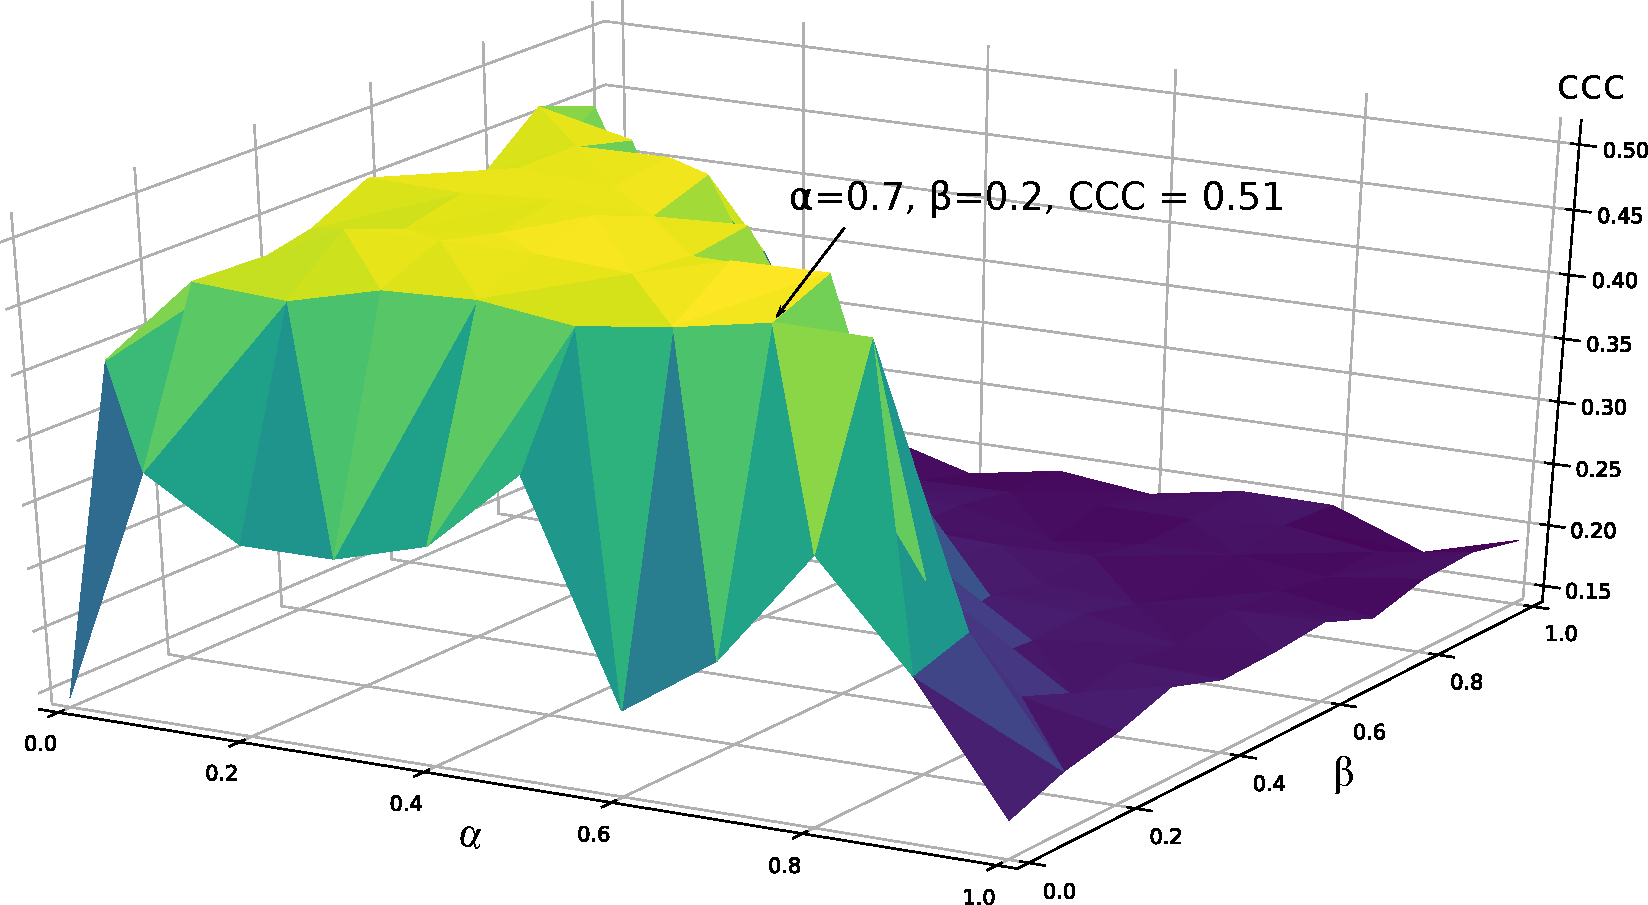
\includegraphics[width=0.8\textwidth]{../fig/alpha_beta.pdf}
  \end{center}
  \caption{Surface plot of different $\alpha$ and $\beta$ factors for MTL with two parameters; the best mean CCC score of 0.51 was obtained using $\alpha=0.7$ and $\beta=0.2$; both factors were searched simultaneously/dependently.}
  \label{fig:ccc_2-params}
\end{figure}

\begin{figure}[htpb]
\centering
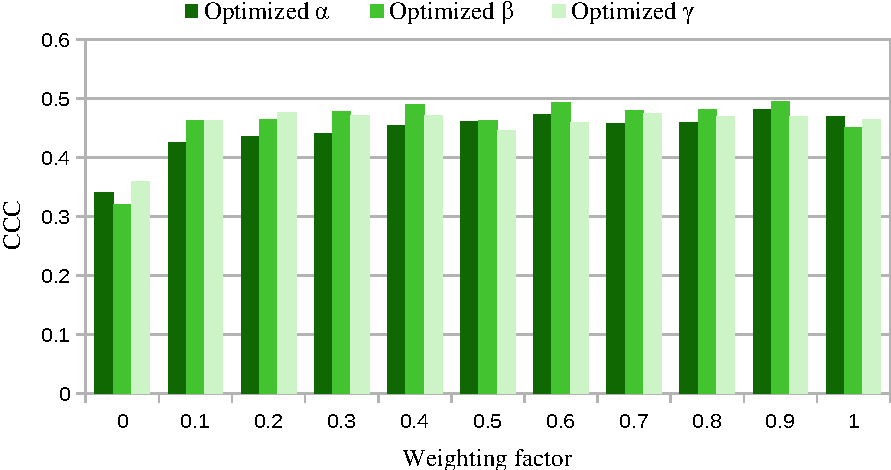
\includegraphics[width=0.8\textwidth]{../fig/alpha_beta_gamma.pdf}
\caption{CCC scores for MTL with three parameters, obtained to find the optimal weighting factors; a linear search was performed independently on each parameter; the best weighting factors for the three parameters were $\alpha=0.9$, $\beta=0.9$ and $\gamma=0.2$.}
\label{fig:ccc_3-params}
\end{figure}

\begin{table*}[htpb]
  \caption{Results of MTL with and without parameters for bimodal feature fusion (LSTM+LSTM); batch size = 256}
  \begin{center}
 \label{tab:mtl-result}
 \begin{tabular}{l c c c c} 
 \hline
MTL method & V & A & D & Mean\\
\hline \hline
No parameter & 0.409 $\pm$ 0.015 & 0.585 $\pm $ 0.011 & \textbf{0.486 $\pm$
0.016} & 0.493 $\pm$ 0.01 \\
2 parameters & \textbf{0.446 $\pm$ 0.002} & \textbf{0.594 $\pm $ 0.003} &
0.485 $\pm$ 0.003 & \textbf{0.508 $\pm$ 0.002} \\
3 parameters & 0.419 $\pm$ 0.012 & 0.589 $\pm $ 0.012 & 0.483 $\pm$ 0.011 &
0.497 $\pm$ 0.008 \\
 \hline
 \end{tabular}
\end{center}
\end{table*}

\subsubsection{Evaluation of dropout for different modalities}
An investigation of the impact of the dropout rate for the acoustic and text
networks in bimodal feature fusion was performed to extend the discussion. In
this evaluation, the dropout rates were varied from each modality before
concatenating them. The goal of the evaluation, at first, was to investigate
the dropout rates for the different modalities.

Figure \ref{fig:dropout} shows the impact of different dropout rates and the
obtained CCC scores. From the figure, using dropout rates of $p=0.1$ and
$p=0.4$ for the acoustic and linguistic networks, respectively, achieved the
best score of $CCC=0.510$. These dropout rates were used to obtain the above
results on the bimodal network. 

From the obtained dropout rates, it is believed that this factor depends on the
size of the feature/input rather than on modality differences. The acoustic
network used the smaller HSF for pAA, a 68-dimensional vector,  compared to the
word embeddings' size of 100 sequences $\times$ 300-dimensional word vectors.
Because the goal of using dropout is to avoid overfitting, it is reasonable
that, on small data, the dropout rate is low, while on larger data, the dropout
rate increases. Hence, in this research, it can be believed that dropout rates
depend on the input size rather than its modality.

\begin{figure}[htpb]
\centering
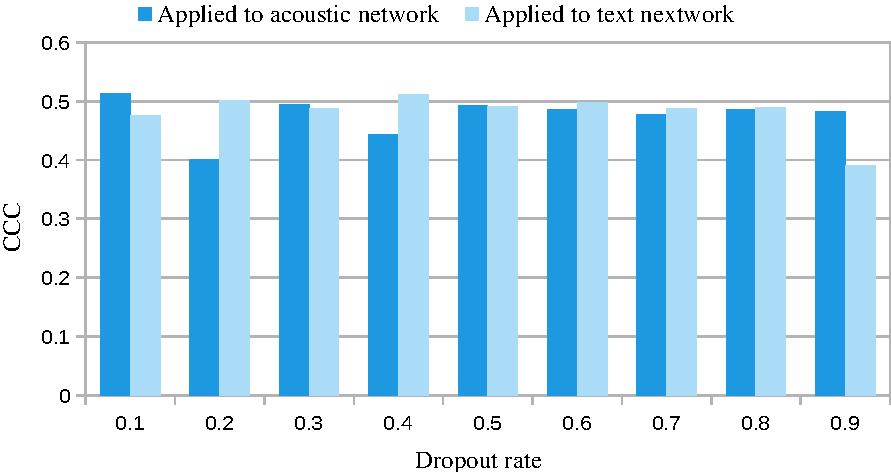
\includegraphics[width=0.8\textwidth]{../fig/dropout_v2.pdf}
\caption{Analysis of dropout rates applied to the acoustic and linguistic networks before concatenating them; the dropout rates were applied independently to either network while keeping a fixed rate for the other network.} 
\label{fig:dropout}
\end{figure}

\subsection{Discussion in terms of categorical emotions}
This study on dimensional speech emotion recognition using bimodal features is
an extension of a similar categorical method. Similarities and differences as
compared to the previous categorical research were found in this study. Here,
the discussion is limited to the best bimodal pairs and the impact of feature
sets from different modalities.

In dimensional speech emotion recognition, more consistent results were
attained. This study observed low variation among the experiments, while the
previous categorical research only used the highest accuracy from many
experiments. Both the categorical and dimensional approaches gained performance
improvement over unimodal emotion recognition by combining acoustic features
and word embeddings.  It was found that LSTM networks on both modalities
performed best in dimensional emotion recognition.  This result was also
supported by a small standard deviation and significant differences with
respect to other results.  In the categorical research, a Dense+LSTM pair
attained the highest result, followed by a Dense+CNN pair. High performances in
some of the 20 experiments with the Dense+LSTM pair were observed. Their average
performance ranked fifth, however, among the eight acoustic-linguistic networks
pairs.  The Dense+CNN pair, which was the second-best in the categorical
emotion research, also ranked second in this dimensional emotion approach. This
result from dimensional emotion recognition was supported by the fact that the
LSTM also attained the highest performance on unimodal emotion recognition.
Similar unimodal results were also observed in the categorical approach, in
which the LSTM architecture performed the best among all the architectures.

The second important finding is the different results between categorical and
dimensional emotion recognition from the feature/modality perspective. Feature
set/modality, which attained the highest performance in the categorical
approach, is different from the dimensional approach. In the categorical
approach with the IEMOCAP dataset, word embeddings gave the highest performance
in the unimodal model, as reported in \cite{Atmaja2019b, Tripathi2018a,
Yoon2019, Sahu2019}. In contrast, in the dimensional approach, acoustic
features' average performance gave better performance over linguistic features.
This phenomenon can be explained by the fact that linguistic features (word
embeddings) contribute to valence more than acoustic features do (see Tables
\ref{tab:acoustic-result} and \ref{tab:text-result}). Though the authors in
\cite{Aldeneh2017} found this result, the authors in \cite{chen2017multimodal,
Eyben2010, Karadogan2012} extended it to find that, for arousal, acoustic
features contribute more than linguistic features do. The results here further
extend the evidence that linguistic features contribute more in valence
prediction, while acoustic features give more accuracy in arousal and dominance
prediction.  Given this evidence, it is more likely that acoustic features will
obtain higher performance than linguistic features in the unimodal case since
they provide better performance for two of the three emotional dimensions. As
suggested by Russell \cite{Russell1980a}, however, a categorical emotion can be
characterized by its valence and arousal only. This relation shows why
linguistic features achieve better performances than acoustic features do on
categorical emotion.

As a final remark for this section, some important findings can be emphasized
in this feature-level fusion of acoustic-linguistic information for dimensional
emotion recognition. Dimensional emotion recognition is scientifically more
challenging than categorical emotion recognition. This work achieved more
consistent results than what it did in categorical emotion recognition. The
combination of LSTM networks for both the acoustic and linguistic networks
achieved the highest performance on bimodal feature fusion, as the same
architecture did on unimodal emotion recognition.  The proposal on using MTL
for simultaneously predicting valence, arousal, and dominance worked as
expected, and it is found that MTL with two parameters represented the
interrelation among the emotional dimensions better than other MTL methods did.

% \section{Comparing ASR outputs with manual transcription}

\section{Dimensional SER with ASR outputs}
In the previous section, the linguistic information provided for the fusion
with acoustic information came from manual transcription. It is difficult to
obtain the linguistic information (i.e., correct transcription of spoken words)
from the speech in a real implementation. Hence, this study evaluates the
fusion of acoustic and linguistic information from ASR outputs to provide
insight into the early-fusion method's achievement with current ASR technology.

Figure \ref{fig:ser_asr} shows an architecture of dimensional SER with ASR
outputs. While acoustic information can be processed directly from speech, the
linguistic information must wait until text transcription are generated by ASR.
This bottleneck between acoustic and linguistic processing is a worth of study
for future research direction.
\begin{figure}[htbp]
  \centering
  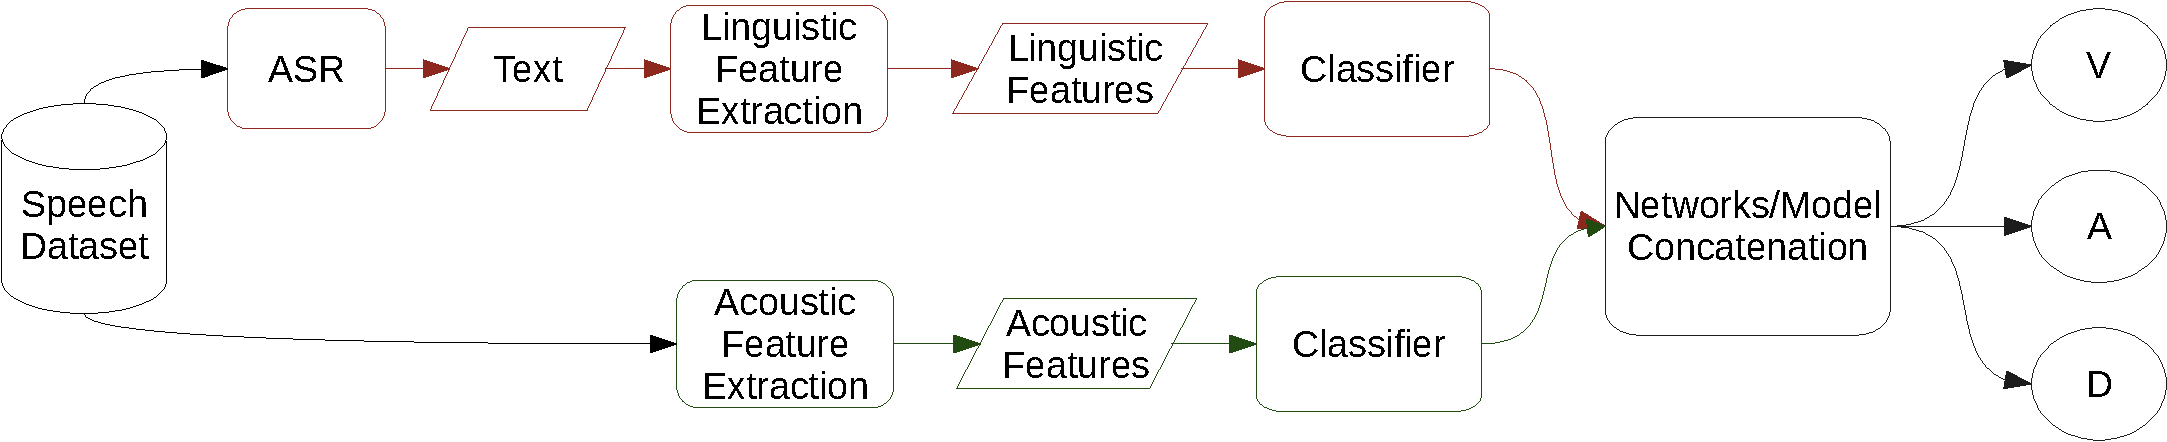
\includegraphics[width=0.9\textwidth]{../fig/ser_asr-crop.pdf}
  \caption{SER architecture by fusing acoustic and linguistic features from ASR outputs}
  \label{fig:ser_asr}
\end{figure}

% Explain the process of transcription
An open-source project, namely DeepSpeech, was used to produce ASR outputs:
text transcription \cite{DeepSpeech2019}. The system was built upon
\cite{Hannun2014}, which used well-optimized end-to-end recurrent neural
networks (RNN) to recognize spoken words. The system achieved a 45\% word error
rate (WER) on the IEMOCAP dataset. This loss in recognizing original (manual)
transcription impacts on the lower performance of linguistic-based dimensional
SER since some words cannot be obtained correctly.

% - Discuss results: TER from ASR outputs
An evaluation of five word embeddings of ASR outputs from IEMOCAP datasets has
been performed. Table \ref{tab:ter_asr} shows the performance of linguistic
information on dimensional SER while Table \ref{tab:serter_asr} shows the
performances of these embeddings when fused with acoustic information. Compared
to manual transcription (Table \ref{tab:text-result}), it is clear that these
results of ASR outputs are worse than manual transcription. There is no
significant difference in the use of pre-trained models compared to the
original word embeddings from these ASR outputs. In this case, the BERT model
achieves the highest performance on linguistic-only dimensional SER.

The addition of linguistic information from ASR outputs only improves the
baseline acoustic information when it utilized pre-trained models. The fusion
of acoustic information (pAA\_D features) with original word embeddings (WE)
attain a lower score than the baseline (average CCC score of 0.4 vs. 0.41). On
the use of ASR outputs, pAA\_D + FastText is the best pair for
Acoustic+Linguistic information from ASR outputs. This highest score from ASR
outputs is 0.05 (10\% of relative loss), lower than the highest in manual
transcription (0.453 vs. 0.508).


\begin{table}[htbp]
  \caption{Evaluation results on emotion recognition using linguistic information from ASR outputs}
  \begin{center}
  \begin{tabular}{l | c c c c}
  \hline
Feature set & V & A & D & Mean \\
\hline \hline
WE        & 0.212 & 0.303 & 0.351 & 0.288 \\
word2vec  & 0.218 & 0.293 & 0.350 & 0.287 \\
GloVe     & 0.226 & 0.279 & 0.349 & 0.285 \\
FastText  & 0.218 & 0.284 & 0.350 & 0.284 \\
BERT      & 0.220 & 0.300 & 0.360 & 0.293 \\
  \hline
  \end{tabular}
  \label{tab:ter_asr}
  \end{center}
\end{table}

\begin{table}[htbp]
  \caption{Evaluation results on emotion recognition using acoustic and linguistic information from ASR outputs}
  \begin{center}
  \begin{tabular}{l | c c c c}
  \hline
Feature set & V & A & D & Mean \\
\hline \hline
pAA\_D $+$ WE       & 0.221 & 0.550 & 0.428 & 0.400 \\
pAA\_D $+$ word2vec & 0.286 & 0.582 & 0.470 & 0.446 \\
pAA\_D $+$ GloVe    & 0.275 & 0.582 & 0.472 & 0.443 \\
pAA\_D $+$ FastText & 0.277 & 0.602 & 0.479 & 0.453 \\
pAA\_D $+$ BERT     & 0.263 & 0.599 & 0.469 & 0.444 \\
  \hline
  \end{tabular}
  \label{tab:serter_asr}
\end{center}
\end{table}

% - Discuss results: SER+TER from ASR outputs

\subsection{Effect of word embeddings' dimension}
Since it is observed that BERT attains the highest performance on
linguistic-only dimensional SER from ASR outputs, a higher dimension of word
embedding may lead to better performance for dimensional SER from linguistic
information. A BERT model has 768-dimension while others have 300-dimension. An
investigation for the effect of word embeddings dimension has been performed by
varying the original word embedding to 768- and 1024-dimension. Table
\ref{tab:ter_we_dim} shows the difference of word embeddings dimension on
linguistic and Acoustic+Linguistic dimensional SER performances. While the use
of a higher dimension shows no significant differences in linguistic-only
dimensional SER, the use of 768- and 1024-dimension improve the
Acoustic+Linguistic pairs (pAA\_D with original WE) to surpass the baseline
acoustic-only (pAA\_D) performance. The larger inputs (WE) may help the network
to learn better to achieve these results.

\begin{table}[htbp]
  \caption{Evaluation of different word embeddings' dimensions}
  \begin{center}
  \begin{tabular}{l | c | c c c c}
    \hline
Feature set & Dimension & V   &   A &   D   &   Mean \\
\hline \hline
WE          & 300   & 0.212   & 0.303 & 0.351 & 0.288 \\
& 768   & 0.199   & 0.307 & 0.352 & 0.286 \\
& 1024  & 0.203   & 0.293 & 0.347 & 0.281 \\
pAA\_D + We & 300   & 0.221   & 0.550 & 0.428 & 0.400 \\
& 768   & 0.255   & 0.596 & 0.464 & 0.438 \\
& 1024  & 0.239   & 0.564 & 0.450 & 0.418 \\
    \hline
  \end{tabular}
  \label{tab:ter_we_dim}
  \end{center}
\end{table}

\section{Early fusion by network concatenation}
\subsection{Bimodal acoustic-linguistic feature fusion}
To evaluate a different approach for early-fusion dimensional SER by fusing
acoustic-linguistic information, this study employs another dataset, the Ulm
State of Mind in Speech-elderly (USOMS-e) corpus. The dataset is part of
INTERSPEECH 2020 ComParE challenge \cite{Schuller}. The task is to predict
categories of valence and arousal, which is converted from a 0-10 scale to low
(0-6), medium (7-8), and high (9-10) classes.

In the previous chapter, an evaluation of acoustic-only valence and arousal
predictions were evaluated. It is shown that feature-based aggregation is
better than the outputs-based aggregation (majority voting). Since the feature
aggregation's goal is to have the same dimension ($n \times 1$) for both
acoustic and linguistic features, it is easy to concatenate both features to
improve valence and arousal prediction. Figure \ref{fig:feature_fusion} shows
an approach on acoustic-linguistic features fusion.  Two feature sets are
stacked horizontally to build a new feature vector for the SVM classifier's
input. 

\begin{figure}[t]
  \centering
  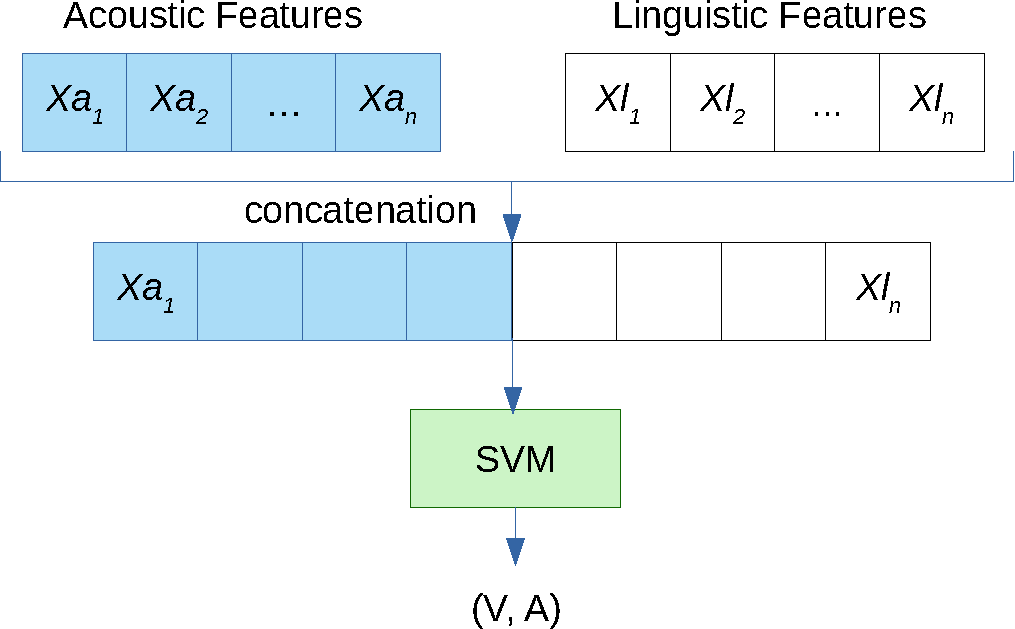
\includegraphics[width=0.7\linewidth]{../fig/feature_fusion.pdf}
  \caption{Acoustic-linguistic feature concatenation with SVM}
  \label{fig:feature_fusion}
\end{figure}

\subsection{Feature concatenation results}
Given a set of acoustic-linguistic features pair ($x_a$ and $x_l$) with valence
and arousal category labels ('L', 'M', 'H'), the task of SVM is to classify
whether a given feature set belongs to a category of valence and arousal. This
classification task is performed using support vector classification (SVC) in
scikit-learn toolkit \cite{scikit-learn} with a linear SVC kernel, $10^6$ of
maximum iteration, and optimized complexities (C) values in the range
[$10^{-6}, 10^1$] with $10^{1}$ step size. For data balancing, imbalanced-learn
toolkit was used \cite{Lemaitre2017}; however, no significant difference was
found between balanced and imbalanced data. The other parameters are left as
default. The SVC classification is performed separately to predict valence and
arousal categories for the same feature set.


Table \ref{tab:bimodal_result} shows the results on using acoustic-linguistic
feature concatenation for valence and arousal category prediction on
development and test partitions. This study improved the UAR score on
development partition from 49.2 to 58.2 for valence and from 40.6 to 52.5 for
arousal. On test partition, the UAR scores were improved from 49.8 to 56.3 for
valence and from 49.0 to 50.4 for arousal. Although the gain was small, it is
shown that bimodal acoustic-linguistic feature concatenation improved the UAR
scores of valence and arousal in most combinations of acoustic-linguistic
feature pairs. Table \ref{tab:bimodal_result} shows that evidence on both
development and test partitions.

\begin{table}
  \caption{Result of bimodal valence and arousal prediction on development and test partition: official baselines vs. proposed method}
  \label{tab:bimodal_result}
  \begin{center}
  \begin{tabular}{l l c c c c}
    \hline
\multicolumn{2}{c}{Features} & \multicolumn{2}{c}{Dev} &
\multicolumn{2}{c}{Test} \\
Acoustic  & Linguistic  & V & A & V & A \\
\hline \hline
ResNet50 \cite{Schuller}  & - & 31.6  & 35.0  & 40.3  & \textbf{50.4}\\
- & BLAtt \cite{Schuller} & 49.2  & 40.6  & 49.0  & 44.0 \\
LibROSA & Gmax  & \textbf{58.2} & 34.6  & 40.5  & 34.8 \\
ResNet50  & Gmax  & \textbf{58.2} & 51.0  & 40.9  & \textbf{50.4} \\
ResNet50  & BLAtt & 47.6  & \textbf{52.5} & \textbf{56.3} & 46.4 \\
BoAW-250  & BLAtt & \textbf{58.2} & 44.4  & 49.0  & 47.4 \\
\hline
  \end{tabular}
\end{center}
\end{table}


\section{Summary}
This chapter reports an investigation of using acoustic features and word
embeddings for dimensional speech emotion recognition with multitask learning
(MTL). First, it can be concluded that using acoustic features and word
embeddings can improve the prediction of valence, arousal, and dominance. Word
embeddings help improve valence prediction, while acoustic features contribute
more to arousal and dominance prediction. All the emotional dimensions gained
prediction improvements on bimodal acoustic and linguistic networks; the
greatest improvement was obtained using LSTM+LSTM architectures pair. Second,
the proposed MTL with two parameters could improve all emotional dimensions'
prediction compared to MTL with no parameters. The weighting factors given to
valence and dominance may represent the interrelation among the emotional
dimensions. This formulation only partially represents that interrelation
because the obtained improvement was still small. The formulation can be
improved for future research by implementing other strategies, particularly
those based on psychological theories and experiments.  Third, a mismatch
between categorical and dimensional emotion recognition can be explained as
follows. Linguistic-based emotion recognition obtained better results than
acoustic features did in categorical emotion, but the result was the opposite
for dimensional emotion. This contrast can be explained by the fact that
categorical emotion only relies on the valence-arousal space. The higher
valence prediction obtained by word embeddings may result in better categorical
emotion prediction than the prediction by acoustic features. Fourth, in
comparing manual transcription with ASR outputs, a 10\% loss in CCC score was
obtained using a word error rate of 45\%. Fifth, the feature concatenation of
acoustic and linguistic features on the USOMS-e dataset obtained higher
performances than a single modality emotion recognition. This feature
concatenation was performed using acoustic features aggregation explained in
the acoustic features side from the previous chapter.

In summary, a combination of speech features and word embeddings can solve the
drawback of dimensional speech emotion recognition. Word embeddings improve the
low score of the valence dimension in acoustic-based speech emotion
recognition. The combination of both features not just improved valence but
arousal and dominance dimensions too. Multitask learning also works as
expected; it can simultaneously predict three emotion dimensions' degrees
instead of predicting one by one dimension using single-task learning. This
strategy may similar to human bimodal emotion perception from voice and
linguistic information. Based on the obtained performances, however, there is
room for improvement, e.g., a fine-tuned BERT model may improve the current
results.  In the next chapter, another framework fusion is explored, i.e., a
late-fusion based approach.
